\documentclass[12pt,a4paper]{book}
\special{papersize=210mm,297mm}
\usepackage{lmodern}
\usepackage[T1]{fontenc}
\usepackage[spanish]{babel}
\usepackage{ragged2e}
\usepackage{biblatex}
\usepackage{csquotes}
\usepackage{graphicx}
\usepackage[hidelinks]{hyperref}
\usepackage[acronym]{glossaries}
\title{Trabajo Final}
\author{Antoniak, Rodrigo Lionel}
\date{2022}
\hypersetup{
    bookmarksopen=true,
    pdftitle={Trabajo Final},
    pdfpagemode=UseThumbs,
}
\urlstyle{same}
\graphicspath{ {./images/} }
\makenoidxglossaries
\renewcommand{\glsnamefont}[1]{\makefirstuc{#1}}
\newacronym{ilc}{ILC}{Instituto Línea Cuchilla}
\newglossaryentry{reldoc}
{
  name={relevo docente},
  plural={relevos docentes},
  description={Cambio de la persona que cumple un rol
  determinado en cierto momento, causado por dos
  posibles motivos; uno es la suplencia del docente
  por una licencia, y otro es el reemplazo del
  titular por renuncia a un cargo específico}
}
\newglossaryentry{coordesc}
{
  name={Coordinación Escolar},
  description={Sección dentro del \acrlong{ilc}
  que cumple el rol de secretaría en el área
  pedagógica, así no se confunde con la sección
  de Administración (parte del área general del
  colegio)}
}
\newglossaryentry{modulo}
{
  name={módulo},
  description={Horario de práctica profesional que
  realizan los alumnos en los sectores correspondientes
  para la actividad. Los lugares pueden ser el taller o
  la carpintería (área técnica electromecánica), la
  granja o el tambo (área agrotécnica), u otros asignados
  para el Bachiller en Turismo}
}

\begin{document}
	\frontmatter
	\pagenumbering{gobble}
	\begin{center}
	{\fontsize{30pt}{36pt}\selectfont \textbf{S.A.E.S.}}
	\newline
	\large{Sistema de Administración para Escuelas Secundarias}
	\newline
\end{center}
\huge{\underline{Universidad:} UNaM}
\vspace{18pt}
\newline
\huge{\underline{Facultad:} FCEQyN}
\vspace{18pt}
\newline
\huge{\underline{Carreras:} Analista en Sist. de Comp.}
\vspace{9pt}
\newline
\huge{Licenciatura en Sist. de Información}
\vspace{18pt}
\newline
\huge{\underline{Cátedra:} Trabajo Final}
\vspace{9pt}
\newline
\huge{Proyecto de Software}
\vspace{18pt}
\newline
\huge{\underline{Alumno:} Antoniak, Rodrigo Lionel}
\vspace{18pt}
\newline
\huge{\underline{Profesores:}}
\newline
\huge{Kuna, Horacio Daniel}
\newline
\huge{Caballero, Sergio Daniel}
\newline
\huge{Rey, Martin}
\newline
\huge{Yatchesen, Facundo}
\vspace{18pt}
\newline
\huge{\underline{Año:} 2022}

	\cleardoublepage
	\pagestyle{plain}
	\pagenumbering{Roman}
	\setcounter{page}{3}
	\tableofcontents
	\listoffigures
	\listoftables
	\cleardoublepage
	\mainmatter
	\pagestyle{headings}
	\pagenumbering{arabic}
	\setcounter{page}{13}
	\part{Introducción}
	\LARGE{ \indent
Este trabajo práctico integrador se ha realizado
con el objetivo de completar las cátedras de
Trabajo Final y Proyecto de Software (en el año 2022),
perteneciendo a las carreras de Analista en Sistemas
de Computación y Licenciatura en Sistemas de Información;
correspondientes a la Facultad de Ciencias Exactas,
Químicas y Naturales, que ofrece la Universidad Nacional
de Misiones.
}
\newline
\LARGE{ \indent
En él, se desarrolla el ciclo de vida del desarrollo de
software que corresponde a un sistema de gestión para
para escuelas secundarias (más específicamente, el
\acrlong{ilc}); cuya propuesta se espera poder concretar
para finalizar la carrera de Analista en Sistemas de
Computación, así como avanzar en la Licenciatura en
Sistemas de Información.
}

	\part{Planificación}
	\chapter[Entrevistas]{Planificación de entrevistas}
	\normalsize{ \indent
Primero, se investigó sobre los antecedentes del colegio;
para lo cual, fue necesario realizar una primera entrevista
para averiguar detalles históricos del manejo de información.
Teniendo en cuenta que el problema inicial resultaba ser
muy grande para el tiempo que se dispone, se recolectó
más datos de los necesarios. Toda la información respecto a
este asunto se encuentra en la descripción del escenario.
}
\newline
\normalsize{ \indent
El paso siguiente fue establecer los objetivos de las
entrevistas (se han llevado a cabo dos), las cuales tienen
enfoques distintos por la información que se manejaba del
colegio y por el asentamiento del alcance de la solución.
Para la entrevista número uno, se propuso como objetivos:
}
\begin{itemize}
  \item Conocer los antecedentes del colegio con el
  gestión de docentes y alumnos (si bien, esto puede
  resultar recursivo en el trabajo práctico; es la realidad
  de la situación, ya que lo único que se conocía antes de
  la entrevista era el deseo de tener un gestor de legajos
  y formularios).
  \item Informarse sobre los problemas que posee la escuela
  secundaria respecto a legajos y formularios. Además,
  constatar si existe algún tipo de solución sugerida por
  los futuros clientes del sistema.
  \item Comprobar si las sugerencias generadas por el
  entrevistador para el sistema son viables para los
  entrevistados. Es decir, si las ideas de la posible
  solución son convenientes para la solución que se genere
  (al menos, según los clientes del futuro software).
  \item Recolectar datos sobre los procedimientos para
  legajos y formularios.
\end{itemize}
\ \newline
\normalsize{ \indent
Para la entrevista más reciente, con un alcance ya definido;
han surgido nuevos objetivos de la entrevista, los cuales son:
}
\begin{itemize}
  \item Investigar la clasificación de los docentes según el
  horario.
  \item Identificar los derechos que los usuarios finales
  tienen sobre el software.
  \item Recolectar datos para analizar las condiciones
  necesarias para registrar a los docentes.
  \item Establecer las reglas a cumplir sobre las horas
  cátedra, el cambio de horarios y el \gls{reldoc} (tanto
  por licencia como renuncia a las horas).
  \item Averiguar el método de asistencia y calificaciones
  que se encuentra actualmente en la institución.
  \item Definir el carácter de la solución frente a las
  distintas situaciones que se puedan presentar.
\end{itemize}
\ \newline
\normalsize{ \indent
A continuación, debía decidirse a las personas que serían
entrevistadas; sin embargo, es necesario dar contexto del
tiempo en que se iban a llevar a cabo los encuentros. A las
fechas de realización del trabajo práctico integrador de
ingeniería I (del cual se extrae parte de este trabajo), el
mundo no se encontraba en una situación normal; el virus
COVID-19 estaba en circulación, por lo que el personal que
trabajaba era limitado. Teniendo en cuenta esto, por descarte
ha resultado que sólo dos personas estaban disponibles para
realizar la entrevista; además, coincide que ambos sujetos
acceden a la entrevista en simultáneo. Cabe destacar que ellos
pertenecen a Coordinación Escolar, tal y como se pretendía
inicialmente (sin tener en cuenta el asunto de coronavirus);
la razón es que son el sector que administra los asuntos
relacionados a legajos, formularios, información personal,
horarios, relevamientos, entre otros.
}
\newline
\normalsize{ \indent
Luego, el autor de este documento se encargó de preparar a los
entrevistados; dando una guía del material que se podía
solicitar en conjunto con los asuntos de las preguntas a
darse. Entre los documentos recibidos, se encuentran los
requisitos para legajos de docentes y alumnos (impreso),
la declaración jurada de los docentes (tanto en papel como
un archivo digital), algunos formularios (los cuales no son
de interés, a causa del alcance que se tiene en esta primera
etapa) y el archivo Excel de horarios (no era necesario
obtener el de legajos, bastaba con la observación; dado que
es muy poco efectivo y excesivamente complejo de visualizar,
incluso de forma personal y con detenimiento).
}
\newline
\normalsize{ \indent
Por último, fue momento de tomar una postura ante el tipo
de preguntas y su estructura. Sobre el primer tema mencionado
en este párrafo, se distingue el uso de preguntas abiertas,
cerradas y sondeos para ambas entrevistas. Por otra parte,
la estructura elegida para cada entrevista fue distinta; en
gran parte por la información en el momento que se realizó
cada una.
}
\newline
\normalsize{ \indent
En la primera, se optó por una forma de diamante; comenzando
a indagar sobre diseños que puedan ser parte de la solución
(sea tabla, lista u otro), los métodos de comunicación entre
los usuarios (si los hubiera); el propósito de la acción es
dar una motivación a los entrevistados, ya que así parece ser
que la solución no está muy lejana a la fecha del encuentro y
las personas que contestan las preguntas hacen tal acción con
mayor motivación. Después, se hacen las preguntas más abiertas
para obtener un contexto amplio de la situación; averiguando
los procedimientos y las demandas de los clientes del futuro
software. Al final, se refinan detalles sobre lo discutido
anteriormente para completar la información obtenida.
}
\newline
\normalsize{ \indent
En la segunda entrevista, se optó por una estructura de
pirámide; si bien se informó a los entrevistados sobre el
alcance que se optó en la primera etapa, resultaría más
adecuado adentrar al personal de Coordinación en el tema sin
preguntas amplias. En adición, los datos juntados en la primera
entrevista daban respuesta a muchas de las preguntas específicas
de horarios y relevamientos. Entonces, se ubicaron al principio
preguntas específicas sobre los derechos de acciones de los
usuarios, la clasificación de profesores según horarios y las
reglas correspondientes a cada división (que distingue a cada
categoría). Luego, se prosiguió con la investigación sobre las
asistencias y calificaciones de los docentes y alumnos. Para
concluir, se planifica preguntar sobre el procedimiento de
cambio de horario y relevamiento; en conjunto con sus reglas,
las cuales se suponen que son amplias.
}
\newline
\normalsize{ \indent
Para terminar, cabe mencionar que el uso de sondeos resulta
difícil ubicar en momentos específicos de la entrevista; este
tipo de preguntas se realiza respecto a cierto tipo de respuestas
a una cuestión anterior, por lo que el entrevistador debe prestar
atención al utilizar los mismos en tiempo real. Igualmente, se
tiene una noción de las situaciones clave gracias a la
experiencia.
}

	\chapter[Actividades]{Planificación de actividades}
  \normalsize{ \indent
Para ubicar cada una de las actividades en el tiempo,
se optó por un diagrama de Gantt; con propósitos de ver
las fechas críticas sencillamente, en conjunto con la
existencia de un solo camino transitable. A continuación,
se procede a mostrar el diagrama de Gantt de este documento
(se lo ha dividido en dos partes para favorecer su
visualización):
}
\begin{figure}[!ht]
  \caption{Primera parte de planificación de actividades}
  \centering
  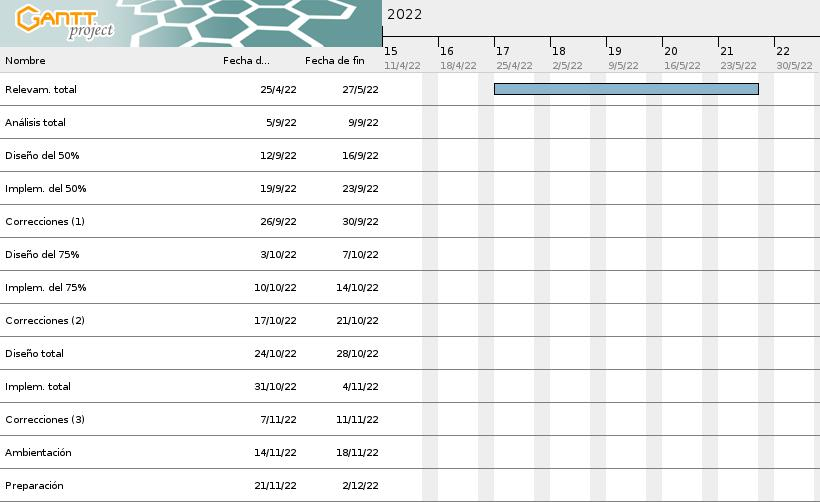
\includegraphics[width=\textwidth]{planTrabajoFinal1}
\end{figure}
\begin{figure}[!ht]
  \caption{Segunda parte de planificación de actividades}
  \centering
  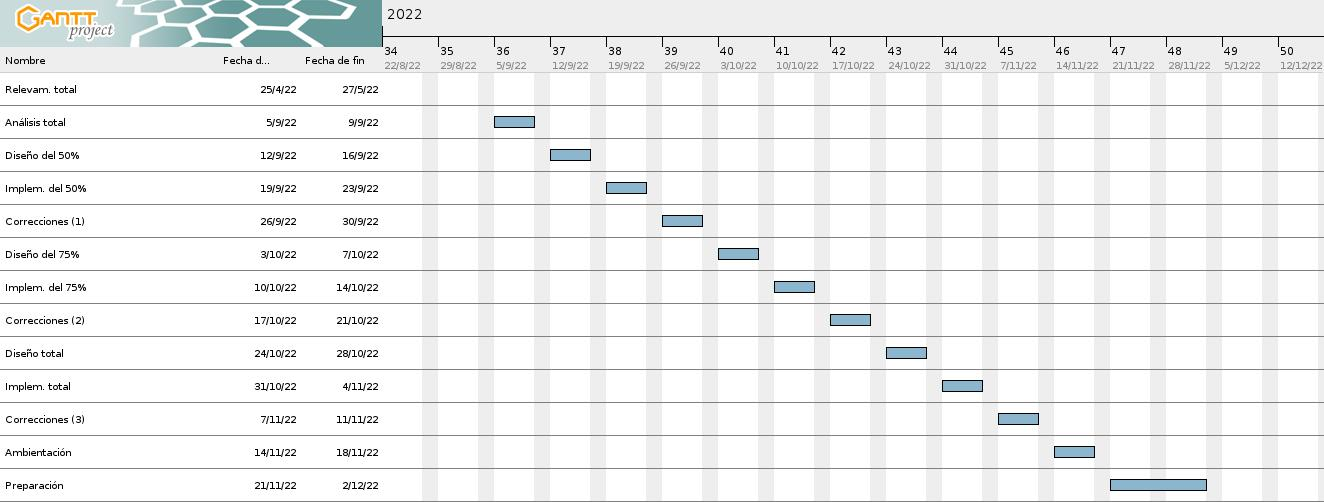
\includegraphics[width=\textwidth]{planTrabajoFinal2}
\end{figure}
\newline
\normalsize{ \indent Consideración:}
\begin{itemize}
  \item Todos los manuales se han estado realizando desde
  el inicio de las actividades hasta el final.
\end{itemize}

	\chapter[Factibilidad]{Estudio de Factibilidad}
  \section[Información]{Información del Proyecto}
\normalsize{ \indent
Sobre el proyecto se obtiene la siguiente información:
}
\begin{tabbing}
  \hspace{1cm}\= \textbf{Nombre}\qquad \qquad \qquad
  \quad \quad \= SAES(Sistema de Administración para
  \\[5pt] \> \> \qquad \quad Escuelas Secundarias) \\[5pt] \>
  \textbf{Tipo} \> Con cliente final\\[5pt] \>
  \textbf{Fecha de preparación} \>
  9 de septiembre de 2022\\[5pt] \>
  \textbf{Cliente} \> Personal del \acrlong{ilc}
  \\[5pt] \> \textbf{Patrocinador} \> \acrlong{ilc}
  \\[5pt] \> \textbf{Líder} \> Rodrigo Lionel Antoniak
\end{tabbing}
\section[Resumen]{Resumen Ejecutivo}
\normalsize{ \indent
Para este proyecto, se pretende desarrollar un
software donde haya una base de datos para almacenar
legajos, horarios, calificaciones y asistencias;
donde tenga un dominio en un sitio web, para así
poder portar el manejo de perfiles en distintas
partes. No ha de tener muchas dificultades respecto
a la competencia, ya que conserva su simplicidad en
el formato que se presenta.
}
\newline
\normalsize{ \indent
Sus puntos principales son el cumplimiento a las
necesidades del colegio, con un formato que favorece
al uso de recursos humanos que ya se poseen y poco
entrenamiento; teniendo que invertir principalmente en
la programación y la base de datos. La tarea que abarque
la totalidad del precio de la solución es la instalación
de software, debido a que se utiliza la licencia GPL v2.
}
\newline
\normalsize{ \indent
Como el diseño es bastante personalizado por el
\acrlong{ilc}, se pretende que el proyecto se realice una
única vez; sin llevarlo a la reventa del programa, o al
menos no es el propósito. Cabe destacar que cada escuela
puede solicitar requisitos distintos, por lo que la
variedad de soluciones es alta para realizar una de
propósito general.
}
\newline
\normalsize{ \indent
Visto y considerando que existe información suficiente
sobre el contexto, podrá llevarse a cabo este proyecto
(o al menos en el alcance pretendido actualmente);
después, será necesario continuar con las buenas prácticas
para completar todo el sistema e integrarlo como espera
el colegio secundario.
}
\section[Antecedentes]{Antecedentes del Proyecto}
\normalsize{ \indent
Primero, los factores que justifican la realización del
proyecto son la ausencia de digitalización de documentos,
el medio de manejo actual de información (a través de Excel)
y el fracaso de personal informático (contratado por freelance)
para realizar correctamente un proyecto funcional efectivo.
De ahí, el estudio de factibilidad es impulsado por las posibles
opciones que existan, la abertura del cliente a distintas
propuestas y la necesidad de decidir si comprar o desarrollar
software.
}
\section[Contexto]{El Proyecto y su Contexto}
\normalsize{ \indent
Una escuela de nivel medio desea digitalizar la generación
de formularios y completado de legajo. Los docentes y alumnos
pueden completar los datos de sus legajos desde una plataforma,
donde se conservará la información en una base de datos; así
posteriormente se genera el documento y es firmado
presencialmente. El único documento excepcional de esto es la
ficha médica, la cual se ofrece el modelo y se trae el papel
completado por el médico.
}
\newline
\normalsize{ \indent
El acceso a los datos de los legajos será compartido,
aunque estará limitado a aquellos que tengan el rango
suficiente para acceder a la información. Los legajos
podrán observarse desde el perfil del alumno o docente,
o en una tabla que junte a los cursantes o los profesores.
Los docentes pueden clasificarse por el tipo de salario
(por hora, cargo, o ambos), mientras que los alumnos se
pueden clasificar por curso/año/división.
}
\newline
\normalsize{ \indent
Entre otros, debe disponerse de un control de horarios;
propuesto para que la Rectora pueda asignar los docentes
correspondientes a cada rol y el sistema ajuste los
horarios del mismo. Cuando se necesite cambiar los
horarios, el sistema debe controlar que se cumplan todas
las condiciones para la operación. A su vez, la opción de
un docente suplente (dado por la licencia del titular) es
fundamental en el sistema; igualmente que el cambio de
docentes en medio del año.
}
\newline
\normalsize{ \indent
Además, debe permitir registrar asistencias con los
alumnos y docentes de forma directa; así, se libera
al preceptor para que se encargue de otros trabajos.
Cada presente abarcará la condición de un alumno
con las horas contínuas de una materia determinada,
implicando que tras el cambio de materia o la descontinuidad
de una misma materia debe contabilizarse como una asistencia
aparte.
}
\newline
\normalsize{ \indent
Por otro lado, es necesario almacenar las calificaciones
entre docentes y alumnos; tanto las que reciben estos
últimos por su desenvolvimiento en el cursado, como del
profesor por la calidad de enseñanza que otorga. El primer
tipo de calificación requiere que sea trimestral, en donde
cada materia de ese lapso debe tener 3 calificaciones cada
uno. Mientras que las devoluciones de alumnos a docentes
se realiza anónimamente de forma aleatoria.
}
\newline
\normalsize{ \indent
El sistema debe poder generar notificaciones para
informar sobre el estado de cada uno de los estados del
sistema, independientemente del perfil que se involucre.
El motivo del aviso sobre documentación puede ser la falta
de los mismos para completar el legajo o que se notifique
de estar al día, a su vez que puede destacar algún tipo de
error en los datos ingresados en un formulario en específico.
Adicionalmente, los docentes recibirán un correo a través del
dominio del colegio.
}
\newline
\normalsize{ \indent
En adición, existen otros formularios que pueden
generar los miembros por temas distintos al legajo;
entonces se necesitará un canal distinto de gestión
para esos documentos. Incluso, se deberán incluir
documentos históricos; teniendo en cuenta papeles
anteriores a la creación del sistema, siguiendo un
orden lógico de ubicación (sea por fecha, alumno,
curso, etcétera).
}
\newline
\normalsize{ \indent
Por último, debe haber un apartado donde se administren
los exalumnos; teniendo sus nombres, datos de graduación
(año/título) y contacto. Idealmente, cada uno de los
egresados podría cambiar datos de su contacto; así el
colegio puede conservar contacto con ellos. Si bien,
puede evaluarse un sistema de mensajería por el software;
el colegio insiste en tener medios alternativos, con
motivos propios del ente.
}
\newline
\normalsize{ \indent
Respecto al contexto, se puede mencionar que el autor
de este trabajo final ha cursado su nivel medio en este
colegio; lo cual, facilita la comunicación con los
miembros del establecimiento. Tomando en cuenta el
diálogo en la entrevista, puede afirmarse que hubo
acuerdo en la visión de cada miembro de Coordinación
Escolar entrevistado.
}
\section[Alcance]{Alcance del Estudio de Factibilidad}
\normalsize{ \indent
El alcance pretendido para este estudio es el conocimiento
de los pasos a seguir para poder gestionar legajos,
horarios, calificaciones y asistencias. Principalmente,
se analizarán distintas opciones por los costos de
almacenamiento y dinero para elegir; considerando que debe
cumplirse la condición de poder usar el personal ya
contratado del colegio con la posible solución.
}
\section{Factibilidad Técnica}
\normalsize{ \indent
En la búsqueda de las distintas soluciones,
se han encontrado distintas herramientas que
parecen ser candidatas a ser parte del software
final. Para la investigación inicial, se enfocó
en encontrar soluciones destinadas a escuelas;
donde se incluya el manejo de legajos y horarios
docentes. Además, se recuerda que el colegio ya
posee el software de Acadeu; tras el suceso de que
el software no satisface las necesidades del
\acrlong{ilc}, se debe módulos de calificaciones y
asistencia. Gestionar tareas para alumnos debe 
revisarse para un proyecto a futuro, considerando
que la vuelta a la normalidad (frente a la situación
del COVID-19) permite la entrega presencial de
tareas y se insiste en conservar este método.
}
\newline
\normalsize{ \indent
Con todos los filtros establecidos, se destaca un
proyecto de código abierto (bajo licencia pública de
GNU); se llama Proyecto ALBA, aunque ya fue abandonado.
Consiste en la gestión de unidades educacionales, junto
con sus alumnos y docentes; destacándose que existen
módulos para gestionar legajos y horarios docentes. El
asunto es que no parece ser muy conocido y no tuvo mucha
atención, ya que todos los problemas reportados no fueron
respondidos (y quedaron abiertos). Incluso, su página web
principal ya no existe; empero su enlace por GitHub sigue
siendo accesible (como archivado), el cual es el siguiente:
\url{https://github.com/proyectoalba/alba}.
}
\newline
\normalsize{ \indent
Por lo tanto, se observa que no hay una opción íntegra
que cumpla con lo pretendido en el alcance del proyecto;
así que se ha buscado las funcionalidades por separado, en
caso que existiera una herramienta disponible. Si bien, para
la administración de horas docentes se encuentran herramientas
con propósitos laborales generales; no hay alguna que se centre
solamente en gestionar horarios, es decir que trae muchas otras
funcionalidades no deseadas. Se puede nombrar de ejemplo a
PlanningPME
(\url{https://www.planningpme.es/software-planning.htm})
y Sesame (\url{https://www.sesametime.com/}). Para la
gestión de legajos, asistencia y calificaciones; se considera
que la funcionalidad es suficientemente genérica como para
poder generar el código sencillamente y que se enfoque en
solucionar específicamente lo deseado.
}
\section{Factibilidad Económica}
\normalsize{ \indent
Este factor puede resultar esencial hasta cierto punto,
pero hay consideraciones a tomar que bajan la importancia
de este factor:
}
\begin{itemize}
  \item Este proyecto no se pretende volver a usar, ya que
  el colegio nos ha elegido en criterio a la relación de 
  alumno (por el autor de este documento); mas falta decir
  que deja de ser un proyecto cuando se vuelve a realizar.
  Otros colegios pretenderían buscar otras características,
  por lo que sería un proyecto aparte.
  \item El \acrlong{ilc} tiene predisposición a pagar precios
  elevados, siempre y cuando se cumpla con la funcionalidad
  buscada. Además, tiene conocimientos sobre los precios
  reales de software (ya se comentó antes que intentaron
  tener este proyecto resuelto antes con otras personas, pero
  estos últimos no estuvieron a la altura de las
  circunstancias).
  \item Dado que el personal se pretende conservar y que no
  se necesitará mucho entrenamiento, gracias a que se sigue
  el formato que ellos desean con los procedimientos
  adecuados para \Gls{coordesc}; los únicos elementos
  a cobrar son la base de datos, el dominio y la programación.
\end{itemize}
\ \newline
\normalsize{ \indent
Dado que no se conoce la programación requerida, resulta
imposible estimar en este tiempo el costo en sí; sin embargo,
no resulta tan relevante frente a otros proyectos con
competencia y recursos financieros muy limitados.
}
\section{Factibilidad Legal}
\normalsize{ \indent
Tomando en cuenta que se pretende hacer uso de una base de
datos para almacenar los datos sobre los docentes (contando
sólo esta etapa), debe considerarse el manejo de los datos
personales; cuya protección está normalizada en la ley 25326,
que se encuentra en el siguiente enlace:
\url{http://servicios.infoleg.gob.ar/infolegInternet/anexos/60000-64999/64790/norma.htm}.
}
\newline
\normalsize{ \indent
De ahí, hay que tener énfasis en el artículo 10; en
consecuencia, el secreto profesional de los datos personales
es obligatorio (incluso después de terminar la solución
completa).
}
\section{Factibilidad de Recursos}
\normalsize{ \indent
Desde el inicio del proyecto, se tuvo la visión de un relevo
de métodos para realizar operaciones; y no de agregar más
trabajo para hacer, por lo que se aplicó esfuerzo en
limitarse con los recursos ya existentes del colegio.
Gracias a que el personal de \Gls{coordesc} ya realiza
todas las tareas pretendidas con este sistema, aunque con
una forma poco efectiva; no se necesitará agregar personal
para este sistema, ni se afecta a ninguna operación (por lo
que no hay dependencias ni procedimientos necesarios para
describir).
}
\newline
\normalsize{ \indent
Apartando los recursos humanos ya presentes, es necesario
tener una base de datos para el almacenamiento de datos
sobre legajos y horarios (inclusive también para la
incorporación de los elementos pertenecientes a las
siguientes etapas). Para este proyecto, tanto en el
alcance actual como en su totalidad, es ideal realizar
con un dominio web; por motivos de portabilidad para los
docentes y alumnos, cuando quieran actualizar su perfil.
En caso de elegir un diseño de página web, puede
aprovecharse el dominio ya existente del colegio; el cual
es \url{https://www.ilc.edu.ar/}.
}
\section{Factibilidad de Mercado}
\normalsize{ \indent
Como se ha visto en la factibilidad técnica, existen
varias opciones en el mercado que se acercan a algunas
de las necesidades. Para la gestión de una escuela, hay
muchas opciones que se hallan buscando en Internet; sin
embargo, poseen características que resultan ser
complicadas de implementar en muchos colegios. Por
ejemplo, el seguimiento de asistencia, tomando en cuenta
que el colegio cuenta con una residencia para internados;
en especial, por tener una ubicación biométrica o GPS.
}
\newline
\normalsize{ \indent
Por otro lado, hay aplicaciones que se destinan a la
gestión de horarios; la cual administra hasta las
vacaciones que poseen cada uno de los trabajadores. El
problema es que no gestiona los legajos docentes, así
que lamentablemente no se tiene suficiente
especialización en estas alternativas. En fin, esta
solución a desarrollar va a resultar como una oferta
única en el mercado; aunque se pretende que el
\acrshort{ilc} utilice, sin buscar que otros colegios
puedan pedir tal oferta.
}
\newline
\normalsize{ \indent
Para resumir, este software está pretendido para que
los colegios puedan gestionar la administración pedagógica;
sin tener herramientas complejas de implementar en
regiones no pertenecientes al primer mundo. En principio,
el primer cliente (el colegio secundario que solicitó
nuestra solución) elige nuestro sistema porque va a cumplir
correctamente la función solicitada; sin incorporar
herramientas innecesarias para esta escuela, como otras
ofertas.
}
\newline
\normalsize{ \indent
En otras palabras, la persona que escribe este documento
tendrá una solución que está entremedio de dos tipos de
competencias. Por un lado, están los programadores a nivel
local; quienes no resultan ser suficientemente competentes
para cumplir lo que busca el colegio, según testimonio del
personal del establecimiento. El otro sector es el conjunto
de organizaciones que ofrece demasiadas herramientas para
colegios de regiones lejanas a ciudades como Córdoba.
Ofrece una oportunidad donde se tienen las características
programadas correctamente y mantiene la simplicidad del
mismo, siendo el enfoque de esta solución.
}
\section{Factibilidad Operacional}
\normalsize{ \indent
Dentro de las operaciones que se cumplen, se gestiona
la base de datos con los legajos y horarios. Para los
legajos, se completa el legajo de los docentes por dos
formas; dependiendo de quién haga la carga de los archivos
digitales, sean las imágenes o la declaración jurada
firmada. Una persona puede ser el mismo docente,
rellenando un formulario con información que se
complementa con los cargos asignados, los títulos
superiores y la información básica de perfil; para así
tener el modelo de declaración jurada digital que se
podrá imprimir y firmar para guardarse en la base de
datos. La otra opción es el personal de \Gls{coordesc},
donde éste deberá realizar la carga de la información
del formulario mencionado anteriormente; considerando
que el docente prefiere completar la declaración jurada
a mano.
}
\newline
\normalsize{ \indent
Todo lo explicado con respecto a la declaración jurada
se aplica igualmente con las imágenes, distinguiéndose
la verificación de imagen; en el caso que el docente
suba la imagen por su decisión, ya que no hay seguridad
de que la imagen corresponda al documento solicitado
(incluso, puede tratarse de una confusión de documentación;
donde un docente sube un documento en el lugar que
corresponde a otro).
}
\newline
\normalsize{ \indent
Todo lo explicado con respecto a la declaración jurada
se aplica igualmente con las imágenes, distinguiéndose
la verificación de imagen; en el caso que el docente
suba la imagen por su decisión, ya que no hay seguridad
de que la imagen corresponda al documento solicitado
(incluso, puede tratarse de una confusión de documentación;
donde un docente sube un documento en el lugar que
corresponde a otro).
}
\newline
\normalsize{ \indent
Para los horarios, la Rectora es quien asigna los
docentes que se encargan de los distintos puestos
disponibles; subdividiéndose en horas jornales y cargo,
donde un docente puede tener ambos. Así también, la
Rectora hace los \glspl{reldoc}; sea por una suplencia o
por un reemplazo de titular. De ahí, \Gls{coordesc} se
encarga de ajustar los horarios según las condiciones
necesarias para ello; tanto el ajuste inicial de cada
año como los cambios de horario interanuales.
}
\newline
\normalsize{ \indent
Al elegir un docente para cierto horario, la Rectora
tiene todos los permisos para hacer la operación y no
necesita guiarse de ninguna condición. Por el contrario,
para los horarios existe un conjunto de necesidades a
cumplir para los cambios:
}
\begin{itemize}
  \item Un horario a cambiar de un docente no puede
  sobreponerse a otro del mismo profesional, ya sea en
  el mismo colegio o externamente (dato conocido en la
  declaración jurada).
  \item Para una clase que no corresponda a \Gls{modulo}
  (práctica), no se puede tener más de tres horas
  consecutivas de cátedra.
  \item Las horas de \Gls{modulo} deben ser 7:30 a 12:00,
  9:00 a 12:00 (en ambos casos, con un recreo de 10:00
  a 10:30 y sin actividades después del mediodía), o
  14:00 a 16:30 (sin actividades en adelante).
  \item Los docentes no pueden trabajar más de 42 horas.
  Para los que trabajan fuera del colegio (quienes sólo
  tengan horas jornales), se considera el horario externo.
  \item Las horas correspondientes a un curso no se pueden
  interponer. Por lo tanto, siempre que se cambien horarios;
  resulta en una rotación, donde los horarios involucrados
  pueden ser variables (al menos son dos).
\end{itemize}
\ \newline
\normalsize{ \indent
Adicionalmente, los \Glspl{modulo} no pueden cambiarse de
horario dentro del año.
}
\section{Factibilidad de Tiempo}
\normalsize{ \indent
Considerando que la competencia no cubre las necesidades de
la escuela específicamente, no hay un riesgo aparente del
tiempo frente a otros que puedan hacer la misma tarea en
menor tiempo; porque no se halló a alguien con esos rasgos.
Sin embargo, no hay que olvidarse que uno se compromete con
la entrega del software; por lo tanto, se debe seguir los
tiempos previamente tratados con quien nos vaya a comprar el
sistema.
}
\section{Recomendaciones}
\normalsize{ \indent
Cuando se siga con otros objetivos generales que no se abarcan
en el alcance de ahora, es recomendable conservar las prácticas
actuales; así en el futuro se podrá apuntar al éxito de este
proyecto, el cual ya contempla un gran potencial.
}
\newline
\normalsize{ \indent
Ya que no hay muchas opciones en el mercado que cumplan las
funciones del alcance de forma simplificada, se consiguen los
motivos para llevar adelante el software pretendido. Además,
el acuerdo entre los desarrolladores y el cliente de la forma
final otorga confianza que es una buena idea para seguir.
}
\newline
\normalsize{ \indent
Para finalizar, es muy factible ejecutar el proyecto en
cuestión (al menos, hasta el alcance en esta primera etapa) y
debe continuarse con los procedimientos correspondientes; para
así lograr los objetivos de la solución que se creará.
}

	\part{Relevamiento}
	\chapter[Recolección]{Recolección de Información}
	\section{Primera Entrevista}
\normalsize{ \indent
Con este proyecto, se desea controlar el legajo de
docentes y alumnos, así como que ellos puedan generar
formularios; entre otros, tener seguimiento de los
alumnos graduados del colegio. Para los legajos, podría
haber un seguimiento de cada docente/alumno con una
vista tipo tabla; inclusive, sería mejor tener los
archivos a mano junto con la tabla.
}
\newline
\normalsize{ \indent
Toda la información obligatoria de cada uno se halla en
los legajos, aunque en el futuro se podría necesitar
información extra. Por cierto, si se debe informar sobre
el estado de los legajos, sería únicamente a los docentes
por el correo que les otorga el colegio; se prefiere
informar más personalmente a los padres de los alumnos,
tal como teléfono fijo o celular.
}
\newline
\normalsize{ \indent
No hace falta nombrar todos los formularios de los
docentes y los alumnos, se cree que es suficiente con un
modelo digital de cada uno. Lo que si hace falta mencionar,
es que de los exalumnos se quiere conservar información
sobre su graduación de contacto.
}
\newline
\normalsize{ \indent
Los formularios se rellenan en la actualidad a mano,
aunque los modelos de los mismos se hallan en digital.
Cada vez que se necesite uno, se imprime el modelo y se
completa a mano; para después ser firmado, en caso de ser
necesario.
}
\newline
\normalsize{ \indent
En el sistema, se pretende que los docentes y alumnos
sólo puedan controlar sus legajos, perfiles y formularios.
Para el personal de Coordinación Escolar, se pretende
poder dar seguimiento de todos los legajos y formularios.
Por otra parte, la rectora se encarga de gestionar a los
docentes; designando los cargos y haciendo los relevos
necesarios.
}
\newline
\normalsize{ \indent
Del legajo, se puede digitalizar todas las partes, a
excepción del certificado médico de los alumnos; el cual
debe completar el médico que corresponda a cada uno, para
así guardar una copia digitalizada del mismo. De ahí, se
pueden guardar la información en una base de datos;
evitando que se deba reescribir una y otra vez la
información.
}
\newline
\normalsize{ \indent
Si se implementara algún sistema de comunicación, sería
de notificaciones; ya que existe la plataforma Acadeu,
la cual otorga un medio de comunicación entre los distintos
miembros del colegio. Además, no se pretende el envío de
mensajes entre los usuarios; el enfoque es sobre la gestión
de todo el papeleo en un solo lugar.
}
\section{Segunda Entrevista}
\normalsize{ \indent
Según su salario, los docentes se clasifican en jornales y
cargos; donde ambos roles pueden ser de un mismo docente.
De ahí, la cantidad de horas máxima que puede trabajar un
docente es 42 horas; incluyendo las horas trabajadas fuera
del colegio. Como la rectora es quién maneja los cargos,
ella también autoriza a los mismos; sin importar el título
que tengan en sí, siempre y cuando haya uno superior.
}
\newline
\normalsize{ \indent
Los tipos de relevos docentes que existen son de suplencia
y cambio de titular. La diferencia entre cada uno es que la
suplencia ocurre cuando el titular se halla de licencia,
mientras que el cambio del titular se refiere a una renuncia
de horas de un titular. Si un docente nuevo que releva a otro
por renuncia a las horas, puede que necesite un cambio de
horarios.
}
\newline
\normalsize{ \indent
El manejo de los horarios depende de Coordinación Escolar.
Dentro del año, pueden rotar todos los horarios; excepto
Módulo, el cual sólo tiene una rotación entre alumnos interna
(es decir, no afecta el horario). Para el cambio de horarios,
no se puede tener más de tres horas seguidas de una materia
pedagógica (se excluye Módulo, el cual si tiene más de tres
horas cátedra seguidas); además, el docente a cargo no debe
tener horarios externos que le impidan ejercer el cargo.
}
\newline
\normalsize{ \indent
En la actualidad, los cambios de horario se hacen con una
gestión completa de Coordinación Escolar; por lo cual, deben
revisar todas las condiciones para el cambio de horarios.
En otras palabras, por ahora es necesario revisar todos los
documentos manuscritos para poder controlar que se pueda
cambiar determinados horarios.
}
\newline
\normalsize{ \indent
Considerando todo lo dicho anteriormente, se tiene la mayoría
de razones de por qué se debe tener una validación del sistema
para el cambio de horarios. Lo único que amerita mencionar, es
que se prefiere automatizar completamente la selección de horarios
docentes; ya que puede alivianarse la carga que poseen los
trabajadores de Coordinación Escolar.
}
\newline
\normalsize{ \indent
El método de calificación de los alumnos es del 1 al 10, donde 6 es
la calificación para aprobar. Para el pase del año, los alumnos sólo
pueden tener hasta 3 materias desaprobadas por año. Por trimestre, debe
haber un mínimo de 3 calificaciones; en caso que una materia tenga menor
a ese, deberá contar con esa misma cantidad de todas formas.
}
\newline
\normalsize{ \indent
Los preceptores son los encargados de anotar la asistencia manualmente,
tanto de alumnos como docentes. Esta asistencia debe estar cubierta por
cada hora de cursado que haya, aunque cada presente dado abarca las horas
continuas que tenga una materia.
}
\section{Anexos}
\normalsize{ \indent
En los anexos, se presenta la declaración jurada junto con el
horario de un docente; ambos forman parte de la documentación
manejada dentro del Instituto Línea Cuchilla.
}

	\chapter[Informe]{Informe de Relevamiento}
	\section{Primera Entrevista}
\begin{itemize}
  \item \underline{Alumnos:} En el sistema se desea controlar
  sus legajos y darles la oportunidad de generar formularios a
  los que tengan derecho. Es preferible colocarlos en un formato 
  de tabla, donde se puede ver cada uno de los componentes del
  legajo y si se halla entregado o no; a su vez que puede
  filtrarse por curso y por el estado de sus legajos (completo o
  incompleto). Todos los componentes podrían completarse de forma
  digital, excepto por el certificado médico; lamentablemente, en
  la actualidad sólo se tiene el modelo digital y se escriben los
  campos necesarios a mano. Lo mismo aplica para los formularios.
  Por último, es importante saber que se prefiere mantener la
  comunicación con los alumnos de forma personal; por lo cual no
  habrá un sistema de mensajería, además que ello lo otorga la
  plataforma Acadeu.
  \item \underline{Docentes:} El objetivo del sistema es gestionar
  sus legajos y habilitar formularios para que ellos completen.
  Se busca tener una representación de los legajos en una tabla
  que pueda filtrarse por si se completó el legajo o no. Los
  componentes de sus legajos son digitalizables, pero en la
  actualidad sólo el modelo es digital; ya que se siguen
  completando a mano y conservando el papel como único comprobante,
  tal como los formularios. Sin embargo, es destacable que el
  estado de los legajos se puede notificar a través del correo
  que provee el colegio.
  \item \underline{Exalumnos:} Existe un interés personal en conservar
  datos sobre los alumnos que se hayan recibido en el colegio.
  Principalmente, la información clave de ellos es sobre su egreso y
  formas de contacto.
\end{itemize}
\section{Segunda Entrevista}
\begin{itemize}
  \item \underline{Rectora:} Se encarga del manejo de asignación y
  relevo de docentes. Al principio de año, debe otorgarse cada uno
  de los cargos a los docentes registrados; no necesariamente será a
  todos, porque un docente puede no estar al principio de un año
  determinado. No existe ninguna consideración (más allá de los
  horarios) para asignar los puestos a los docentes, ya que la
  rectora tiene suficientes derechos para hacer las acciones que
  tiene asignadas. De ahí, en medio del año puede haber un relevo de
  docentes; lo cual puede significar una licencia de un docente, o
  una alta y baja del titular.
  \item \underline{Coordinación Escolar:} Se componen de
  coordinadores escolares y secretarios. Ellos se encargan de
  organizar los horarios, tanto al inicio del año como entremedio del
  mismo. El único horario que no tienen derechos para modificar dentro
  del año es Módulo. Por ahora, las asignaciones de horario y los
  cambios se hacen en una tabla de Excel; lo cual es muy inconveniente
  y refuerza la idea de implementar una verificación para los
  movimientos en el horario, considerando que es una operación de alta
  complejidad.
  \item \underline{Docente:} Según su salario, se clasifican en
  jornales y cargos; donde ambos roles pueden ser de un mismo docente.
  En cualquiera de los casos, debe cumplirse la cantidad máxima de 42
  horas del docente; incluyendo las horas trabajadas fuera del colegio.
  De ahí, cuando exista un cambio de horario, no se puede tener más de
  tres horas seguidas de una materia pedagógica (se excluye Módulo, el
  cual si tiene más de tres horas cátedra seguidas); además, el docente
  a cargo no debe tener horarios externos que le impidan ejercer el
  cargo.
  \item \underline{Alumno:} Cada uno recibe 3 calificaciones principales
  por materia de un trimestre, donde una materia que posea una duración
  menor a 3 meses debe seguir esta regla también (sólo para el trimestre
  en que transcurre); al finalizar el año, sólo podrán pasar aquellos que
  tengan a lo sumo 3 materias desaprobadas.
  \item \underline{Preceptor:} Se encarga de colocar la asistencia de
  docentes y alumnos en papel, donde el presente logra abarcar las horas
  contínuas que posea una materia; por cada uno de estos intervalos, es
  necesario realizar este registro.
\end{itemize}

	\chapter[Conclusión]{Conclusión de Relevamiento}
	\normalsize{ \indent
Para el sistema, hay que realizar los siguientes puntos:
}
\begin{itemize}
  \item Digitalizar los legajos, facilitando su gestión a través
  de los docentes y alumnos; por lo que se utilizaría el sistema
  para completar los datos (excepto certificado médico).
  \item Armar modelos de formularios que permita la generación de
  varias instancias del mismo, pudiendo completarlos a través del
  sistema.
  \item Habilitar la subida de un escaneo del certificado médico
  completado y la declaración jurada firmada, como parte del
  legajo.
  \item Establecer una interfaz de tabla para los legajos.
  \item Crear un sistema de notificación del estado de legajos de
  los docentes, enlazándolo con el correo electrónico que le
  provee el colegio.
  \item Posibilitar la carga de graduaciones del colegio anteriores
  a la creación de este sistema.
  \item Permitir a la rectora relevar a los docentes según sus
  criterios.
  \item Habilitar un método de comprobación de validez de horarios,
  a partir de las condiciones de los docentes.
  \item Dar a los empleados de Coordinación Escolar una forma de
  visualizar, establecer y modificar los horarios de los docentes;
  según se necesite, siempre y cuando se respete el punto anterior
  mencionado.
\end{itemize}

	\part{Requisitos}
	\chapter[Escenario]{Descripción del Escenario}
	\normalsize{ \indent
El colegio secundario Instituto Línea Cuchilla realiza
formularios, los cuales corresponden a los alumnos y
docentes; algunos son parte legajo, mientras que otros
son generados por alguno de los miembros. Los papeles que
están en nombre del alumno, tienen gestión de los padres.
Estos documentos se realizan de forma manuscrita (si bien
hay un modelo digital que se imprime, se completan a mano),
por lo que la Coordinación Escolar debe cargar los datos
manuscritos en el sistema que poseen actualmente.
}
\newline
\normalsize{ \indent
Actualmente, se maneja a todos los alumnos y docentes con
una planilla de Excel; donde muestra los datos de cada
miembro, junto con las partes del legajo completas. Además,
los documentos que posee el colegio se hallan sólo en forma
física. Entre otros, el traspaso de información entre los
cargos se realiza cada vez que haya una solicitud de la
misma; ya que no todos tienen acceso a los mismos papeles,
a pesar de tener los derechos a los mismos.
}
\newline
\normalsize{ \indent
Por otra parte, las horas docentes se administran de forma
manual por Coordinación Escolar, donde cada uno posee su
propio horario (refiriéndose a estar impreso en el sector
que corresponde). Al igual que los legajos, el control de
las cargas horarias se realizan a través de una planilla de
Excel; donde constatar la compatibilidad de horarios
(incluyendo las horas que se cumplen fuera del
establecimiento) es tarea que realiza el personal de
Coordinación Escolar, sin ningún tipo de soporte para
validar el cambio de horarios. Cabe destacar que también
así se distingue una suplencia de una alta y baja en un
cargo u hora.
}
\newline
\normalsize{ \indent
En adición, el colegio cuenta con un seguimiento de exalumnos;
donde poseen información de su graduación y contacto. Uno de
los conflictos importantes es que no existe alguna forma de
poder asegurarse de que la información que tiene el colegio es
la actual del graduado, sólo pueden esperar a que la persona se
comunique con el colegio y confirme los datos (junto con su
identidad).
}

	\chapter[Objetivos]{Objetivos del Sistema}
	\normalsize{ \indent
Para el software completo, se proponen los siguientes objetivos
a largo plazo:
}
\begin{itemize}
  \item Poder tener los horarios de los cursos disponibles,
  dentro de la solución final; donde sea posible rotar
  horarios, gestionar licencias, altas y bajas. Es muy
  importante controlar que cada una de estas acciones se
  realice correctamente, siguiendo todas las reglas que tiene
  el colegio respecto a este tema.
  \item Crear una base de datos, donde se tenga los componentes
  necesarios de un legajo docente; con la opción de observar
  éstos de forma ordenada y fácilmente, a la vez tener un acceso
  rápido a la información (sin tener que buscar en una planilla
  de Excel o en carpetas de archivos, ni mucho menos en formularios
  manuscritos).
  \item Tener un apartado dedicado a los documentos históricos que
  existieron antes de la solución propuesta, donde se tendrá un
  ordenamiento eficaz para todo usuario que quiera y tenga permisos
  para acceder a tal información. Inclusive, todos los documentos
  que sean relevados por otros irán a esta sección.
  \item Hallar la forma de digitalizar los documentos posibles;
  así se evita perder tiempo en el paso de datos. Sin embargo,
  cabe destacar que también hay que generar el formulario físico;
  ya que se pretende conservar el método físico.
  \item Sincronizar las notificaciones para los docentes en el
  sistema con el correo electrónico que proporciona el colegio.
  \item Mantener al día la información acerca de los exalumnos
  (si es que ellos lo desean) de la forma más accesible para ellos.
\end{itemize}
\ \newline
\normalsize{ \indent
Por otra parte, para describir el alcance que se presenta en esta
etapa se puede resumir en los dos primeros objetivos escritos en
esta parte. En otras palabras, las metas en este corto plazo son:
}
\begin{itemize}
  \item Establecer las condiciones que limitan el cambio de horarios
  por la jerarquía de importancia, es decir, cuáles son las que
  imposibilitan el movimiento, qué situaciones no tienen las
  validaciones suficientes para rotar (o que necesitan más horas en
  el movimiento cíclico) y cuándo hay derechos para la acción.
  \item Solucionar de forma correcta la situación de un relevamiento
  docente que a la vez debe tener cambios de horario. La causa de
  esto es que Coordinación Escolar controla los horarios, mientras
  que la rectora asigna los cargos.
  \item Crear un formulario digital que sirva para generar la 
  declaración jurada, así se imprime para su firma presencial y se
  almacenan el escaneo del mismo; junto con fotografías de los otros
  requisitos del legajo docente, los cuales pueden subir ellos mismos.
\end{itemize}

	\chapter{Requisitos Funcionales}
	\begin{itemize}
  \item Los docentes podrán completar sus legajos subiendo
  fotografías de la documentación solicitada (excepto la declaración
  jurada), aunque requerirán una validación por parte de Coordinación
  Escolar.
  \item Para la declaración jurada, estará disponible un formulario
  digital para ser completado por los docentes; a partir de la
  información dada, se puede generar un archivo que Coordinación
  Escolar imprimirá al momento que vaya tal docente a firmar
  presencialmente. Por último, el personal de Coordinación Escolar
  se encarga de subir un archivo con los escáneres de los papeles de
  la declaración jurada firmada.
  \item El personal de Coordinación Escolar podrá observar una tabla
  que muestra el estado en que se halla cada uno de los documentos
  del legajo. Se identificarán por 3 colores, cuyos significados se
  explican a continuación. El rojo implica que el Docente no subió la
  imagen del documento o no completó la declaración jurada. El
  amarillo tiene el significado de que la imagen ha sido subida, pero
  debe ser aprobada por Coordinación Escolar; o sino que el formulario
  de la declaración jurada ha sido completado, empero debe subirse tal
  documentación firmada. El verde da a entender que la imagen subida
  ha sido verificada o que Coordinación Escolar subió la declaración
  jurada firmada.
  \item Coordinación Escolar podrá subir las fotografías de los
  docentes que traigan presencialmente el material necesario o quienes
  completen la declaración jurada a mano, aunque es mucho más
  preferible que los docentes completen el último documento mencionado
  de forma digital.
  \item La Rectora tendrá la capacidad de asignar los cargos de las
  horas para cada docente según su criterio. Al principio del año,
  debe elegir obligatoriamente; aunque en medio del año puede hacer
  relevos docentes, ya sea una suplencia o un reemplazo definitivo.
  \item Coordinación podrá asignar los horarios de cada cargo dentro
  de la semana. Cada año, se realiza un cambio de horario obligatorio;
  aunque entremedio pueden existir movimientos de horas. Cabe destacar
  que se deben cumplir las condiciones mencionadas en el estudio de
  factibilidad para rotar horarios.
\end{itemize}

	\chapter{Requisitos No Funcionales}
	\section{Requisito del Producto}
\normalsize{ \indent
Para ejecutarse la página web de forma correcta, los docentes
necesitarán una conexión mínima de 1 Mbps, ya que cuenta con
componentes mínimos para la carga de imágenes y formulario
digital. Por otro lado, la Rectora y Coordinación Escolar
requieren una conexión mínima de 2,5 Mbps; por suerte, en el
colegio se cuenta con WiFi mucho superior a tal cantidad. El
procesador del dispositivo de navegación debe ser de 4 MB de
RAM como mínimo y cada dispositivo accederá al sitio
\url{https://www.ilc.edu.ar/}
para entrar al sistema (se tendrá un subdominio dedicado para
el ingreso a legajos, cargos y horarios docentes; incluso se
puede utilizar el mismo para la totalidad del proyecto).
}
\section{Requisito Organizacional}
\normalsize{ \indent
Cuando se obtienen los datos de la declaración jurada, la firma
debe ser presencial; de tal forma, se verifica que la firma es
real. Además, tener mayor inversión en comprar un sistema de
firma digital que sólo se usaría en el colegio tendría muchos
costos; en consecuencia, se prefiere que al firmar sea en una
hoja física con tinta.
}
\section{Requisito Externo}
\normalsize{ \indent
Se deberá conservar la privacidad de los datos personales
envueltos por secreto profesional. Probablemente, el autor de
este proyecto deba firmar un contrato de confidencialidad para
tener evidencia sobre la manipulación de información de los
docentes.
}

	\part{Análisis}
	\chapter{Diagrama de Casos de Uso}
	\chapter{Casos de Uso Extendido}
	\chapter{Modelo de Dominio}
	\chapter{Diagrama de Secuencia de Sistema}
	\chapter{Contratos}
	\part{Diseño}
	\chapter{Diagrama de Clases}
	\chapter{Diagrama Navegacional}
	\chapter{Diagrama de Interfaz Abstracta}
	\part{Implementación}
	\part{Prueba y Depuración}
	\appendix
	\part{Anexos}
	\chapter[Encuestas]{Encuestas Diseñadas}
	\section{Primera Entrevista}
\begin{itemize}
  \item ¿Se desea controlar el legajo de alumnos y docentes
  solamente?
  \item ¿Sería ideal tener una tabla para ver las condiciones?
  \item ¿Podría enlazarse cada requisito del legajo (su archivo
  en la base de datos) de cada docente/alumno en los campos de
  la tabla?
  \item ¿Hay información extra necesaria de cada perfil? ¿Cuál?
  \item Si hubieran notificaciones sobre el legajo, ¿cuál sería
  el medio ideal para eso?
  \item ¿Cuáles son los formularios que podrán hacer los docentes
  y los alumnos?
  \item ¿Qué información es necesaria sobre los exalumnos?
  \item ¿Por qué se necesita documentación histórica de los
  exalumnos?
  \item ¿Cómo se rellenan los formularios?
  \item ¿Cuáles son las acciones que tendrán permitidas cada uno
  de los usuarios?
  \item ¿Qué partes del legajo pueden digitalizarse?
  \item ¿Es preferible manejar un sistema de notificaciones o
  mensajería directa?
\end{itemize}
\section{Segunda Entrevista}
\begin{itemize}
  \item ¿Cómo se clasifican los docentes, según su salario?
  \item ¿Cuál es la cantidad de horas máximas que puede trabajar
  un docente?
  \item ¿Quién autoriza el rol de un docente?
  \item ¿Qué tipos de \glspl{reldoc} existen?
  \item ¿Qué diferencias hay entre los tipos de relevos?
  \item Un docente nuevo que releva a otro por renuncia a las
  horas, ¿puede necesitar un cambio de horarios?
  \item ¿De quién depende el manejo de los horarios?
  \item ¿Cuáles horarios pueden rotar dentro del año?
  \item ¿Qué condiciones deben cumplirse para el cambio de
  horarios?
  \item ¿Cómo manejan los cambios de horario?
  \item ¿De qué forma verifican actualmente el cumplimiento de
  las condiciones para cambios de horario?
  \item ¿Qué razones podrían haber para que el sistema pueda
  validar cambios de horario?
\end{itemize}

	\chapter[Glosario]{Glosario de Términos}
  \printnoidxglossary[type=\acronymtype,title=Siglas,nonumberlist]
  \printnoidxglossary[title=Definiciones,nonumberlist]
	\chapter{Otros}
	\backmatter
	\chapter{Agradecimientos}
\end{document}
